\def\difficulty{1}
\sujet{Granulometry}\index{Mathematical Morphology!Granulometry}

\begin{note}This tutorial aims to compute specific image measurements on digital images. It consists in determining the size distribution of the 'particles' included in the image to be analyzed.
\end{note}

\noindent The image measurements will be realized on a simulated image of disks and an image of silicon carbide powder acquired by Scanning Electron Microscopy (SEM, Fig. \ref{fig:granulometry:enonce:images}).
\begin{figure}[h]
\centering\caption{These images are used for computing a granulometry of objects by mathematical morphology.}%
\subfloat[Simulated image.]{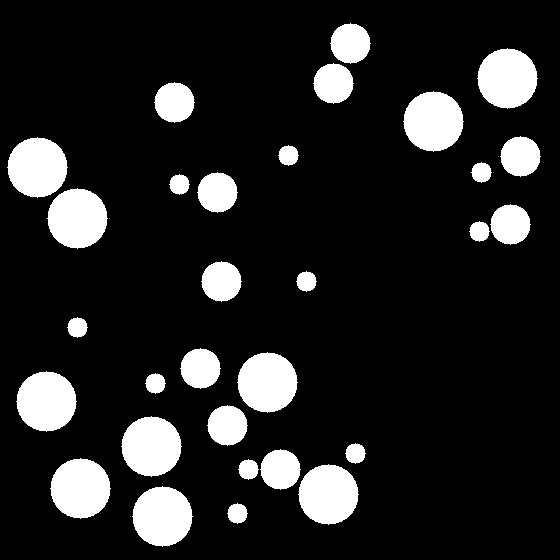
\includegraphics[height=4cm]{simulation.png}}
\hspace{1cm}
\subfloat[Real image of powder, by SEM.]{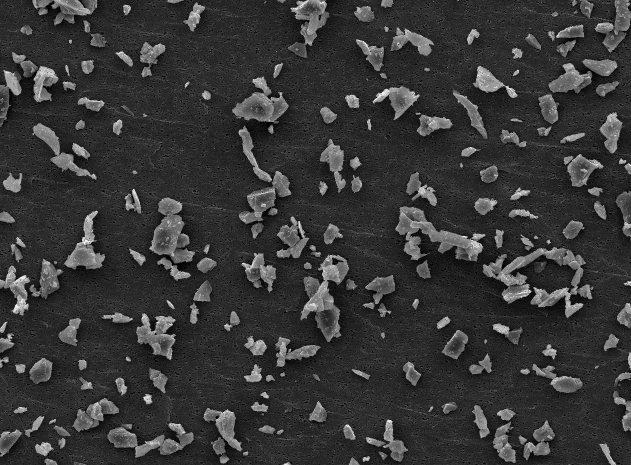
\includegraphics[height=4cm]{poudre.jpg}\label{fig:granulometry:enonce:images:sem}}%
\label{fig:granulometry:enonce:images}%
\end{figure}

\section{Morphological granulometry}
\subsection{Introduction to mathematical morphology}
\iflabelexists{tut:binarymorpho:enonce}{
The tutorial \ref{tut:binarymorpho:enonce} introduces the basic operations of the mathematical morphology, as well as the morphological reconstruction.
}{
The mathematical morphology operations are based upon the Minkowski addition, denoted $\oplus$. If $A$ and $S$ are two sets of an euclidean space $\mathcal{E}$, the Minkowski addition of $A$ and $S$ is the set resulting of the addition of all pairs of elements of $A$ and $S$ (Eq. \ref{eq:stereology:enonce:minkowskiaddition}).

\begin{eqnarray}
 \forall (A,S)\in\mathcal{E}^2, A\oplus S &= \{a+b|a\in A, b\in S \} = \bigcup_{a\in A, b\in S}\{a+b\}\label{eq:stereology:enonce:minkowskiaddition} \\
 \forall (A,S)\in\mathcal{E}^2, A\ominus S &= \{a-b|a\in A, b\in S \} = \bigcup_{a\in A, b\in S}\{a-b\}
\end{eqnarray}

The operations $\delta_S(A)$ and $\varepsilon_S(A)$ respectiveley denote the dilation and the erosion of the set $A$ by the structuring element $S$.
\begin{eqnarray*}
 \delta_S(A) &= A\oplus S \\
 \varepsilon_S(A) &= A \ominus \breve{S}
\end{eqnarray*}

The morphological opening $\phi_S$ and closing $\delta_S$ are respectively defined by:
\begin{eqnarray*}
 \phi_S&=\varepsilon_S\circ\delta_S \\
 \gamma_S&=\delta_S\circ\varepsilon_S
\end{eqnarray*}

These operations are widely used, especially when dealing with the shape of objects, as well as their size. 
} % iflabelexists
More informations can be found in \cite{Soille2003}.

\begin{mcomment}
\begin{mremark}
With Matlab, the useful functions are \minline{imopen} for the morphological opening, \minline{imreconstruct} for the geodesic reconstruction. For counting the number of objects, one can use \minline{bweuler} is the case of objects with no hole, or \minline{bwlabel} for a labelling and counting algorithm.
\end{mremark}
\end{mcomment}
\begin{pcomment}
\begin{premark}
With Python, the useful functions are \pinline{binary_opening} of the module \pinline{scipy.ndimage} for the morphological opening, \minline{binary_propagation} for the geodesic reconstruction. For counting the number of objects, one can use \minline{measurements.label} for a labelling and counting algorithm.
\end{premark}
\end{pcomment}

 
\subsection{Granulometry}
\begin{qbox}
\begin{itemize}
	\item Load and visualize the image 'simulation' Fig.\ref{fig:granulometry:enonce:images}.
	\item Generate $n$ images by applying morphological openings (with reconstruction) to the binary image with the use of homothetic structuring elements of increasing size: $1<\dots<n$.
	\item Compute the morphological granulometry expressed in terms of surface area density. It consists in calculating the specific surface area of the grains in relation with the size $n$ of the structuring element.
	\item Compute the morphological granulometry expressed in terms of number density. It consists in calculating the specific number of grains in relation with the size $n$ of the structuring element.
	\item Compare and discuss.
\end{itemize}
\end{qbox}

\begin{mcomment}
 \begin{mremark}
  Homothetic structuring element can be defined as \minline{se = strel('disk', i, 0)} for disks of size $i$.
 \end{mremark}

\end{mcomment}

\begin{pcomment}
 \begin{premark}
  Use \pinline{generate_binary_structure} and \pinline{iterate_structure} from python module \pinline{scipy.ndimage} to define homothetic structuring elements.
 \end{premark}

\end{pcomment}


\section{Real application}
\begin{qbox}
\begin{itemize}
	\item Load and visualize the image 'powder' of Fig. \ref{fig:granulometry:enonce:images:sem}.
	\item Realize the image segmentation step. I can simply consist in a binarization by a global threshold, followed by hole filling. Noise can also be removed my mathematical morphology opening.
	\item Compute the morphological granulometry (surface area, number).
	\item What can you conclude?
\end{itemize}
\end{qbox}

